\documentclass{LabReport}
\title{操作系统实验报告PA8}
\author{221900180 田永铭}
\date{\today}
\addbibresource{refs.bib}
\Chead{操作系统实验报告PA8 221900180 田永铭}
\Cfoot{\thepage}
\usepackage{listings}
\usepackage{graphicx} 
\usepackage{tikzsymbols}
\usepackage{tikz}
\usepackage{hyperref}

\lstset{
	language=C,               % 语言设置为C
	basicstyle=\ttfamily,          % 设置等宽字体
	frame=shadowbox,               % 代码框
	showspaces=false,              % 不显示空格
	showstringspaces=false,        % 不显示字符串中的空格
	showtabs=false,                % 不显示制表符
	keywordstyle=\color{blue},     % 关键字颜色
	commentstyle=\color{green!50!black},    % 注释颜色
	stringstyle=\color{red},       % 字符串颜色
	numberstyle=\tiny\color{gray}, % 行号颜色
	rulecolor=\color{black},       % 边框颜色
	breaklines=true,               % 自动换行
	backgroundcolor=\color{white}, % 背景颜色
}

\begin{document}
	\maketitle
	
	\tableofcontents
	
	\newpage
	
	\section{实验要求}
	\begin{lstlisting}
// 试在Linux中采用C语言模拟实现Shell中执行如下命令的程序,"cat test1.txt test2.txt | sort"。(可使用如下系统调用: fork, exec, pipe, dup, open, close, wait等)

test1.txt内容:
0
3
5
7

test2.txt内容:
2
6
9
1
	\end{lstlisting}

	\section{实验环境}
	
	\begin{itemize}
		\item 操作系统:wsl2
		\item 编程语言:C语言
		\item 使用工具:gcc编译
		\item 虚拟系统版本:Ubuntu-22.04
	\end{itemize}
	
	\section{实验原理}
	\begin{itemize}
		\item \textbf{Shell中执行该命令的原理:}
		
		需要进行这次实验,首先要了解Shell本身执行该命令的原理:在Shell中,管道操作符`|'用于将一个命令的输出作为下一个命令的输入。例如,命令`cat test1.txt test2.txt | sort'首先执行`cat test1.txt test2.txt',该命令将两个文件的内容连接并输出到标准输出。然后,管道将这个输出传递给`sort'命令,`sort'命令对输入的数据进行排序,并将结果输出到标准输出。Shell通过创建两个子进程来实现这种操作,一个子进程执行`cat'命令,另一个子进程执行`sort'命令。管道在这两个子进程之间建立一个通信通道,使得数据可以从一个子进程流向另一个子进程。
		
		\item \textbf{管道pipe的原理:}
		
		管道是一种常见的进程间通信机制,它提供了一个单向的数据通道,可以在两个进程之间传递数据。管道由内核维护,通常由一个文件描述符对(读端和写端)表示。数据从管道的写端写入,并从管道的读端读取。当一个进程向管道写入数据时,内核会将数据存储在管道缓冲区中,另一个进程可以从管道读取这些数据。如果管道缓冲区已满,写操作会被阻塞,直到有空间可写;如果管道为空,读操作会被阻塞,直到有数据可读。
		
		\item \textbf{dup系统调用的原理:}
		
		`dup'和`dup2'系统调用用于复制文件描述符,使得两个文件描述符指向相同的文件表项。`dup2`更常用,因为它允许指定新的文件描述符的值。例如,`dup2(pipefd[1], STDOUT\_FILENO)'将标准输出重定向到管道的写端,使得后续的输出操作将数据写入管道而不是终端。`dup2(pipefd[0], STDIN\_FILENO)'将标准输入重定向到管道的读端,使得后续的输入操作从管道读取数据而不是终端。通过这种方式,可以在进程之间建立数据流。
		
		\item \textbf{输入输出重定向的原理:}
		
		输入输出重定向通过修改进程的文件描述符表来实现,将标准输入、标准输出或标准错误重定向到文件或管道。例如,通过`dup2'系统调用,可以将标准输出重定向到管道的写端,或者将标准输入重定向到管道的读端。这样,进程的输出将写入管道,另一个进程可以从管道读取输入。这种机制允许将一个进程的输出作为另一个进程的输入,实现数据流的连接。
	\end{itemize}
	
	\section{实验过程}
	\par\hspace{0em}实验主要分为以下几个步骤,其中1是必做,2和3是受到老师启发去探索的:
	
	\begin{enumerate}
		\item 实现输入输出重定向程序
		\item 考察管道的同步机制
		\item 测试创建的匿名管道文件的容量限制
	\end{enumerate}
	
	\subsection{实现输入输出重定向程序}
	
	实验分为三个部分。
	\subsubsection{创建管道}
	
	首先我们需要创建一个管道,搞清楚它的输入端和输出端分别用什么表示,代码如下:
	
\begin{lstlisting}
// 创建管道 fd[0]-读端,fd[1]-写端
int fd[2];
pid_t cat_id, sort_id;
pipe(fd);
\end{lstlisting}

	\subsubsection{创建第一个子进程用以cat}
	
	然后我们需要创建第一个子进程来cat,在这里,我们将cat文件的输出从标准输出设备重定向为输出到管道中,代码如下:
	
\begin{lstlisting}
// 第一次创建子进程,用以cat
cat_id = fork();
if(cat_id == 0)
{
    close(fd[0]); // 关闭管道的读端,关闭不需要的管道读端有助于避免资源泄漏。
	
    dup2(fd[1], STDOUT_FILENO); // 将标准输出重定向到管道的写端
	
    close(fd[1]); // 关闭管道的写端,关闭 fd[1] 有助于防止意外的文件描述符泄漏,并确保子进程结束时,写端被正确关闭,使得读端能够检测到EOF(文件结束)。
    execlp("cat", "cat", "test1.txt", "test2.txt", (char *) NULL);
}
\end{lstlisting}

	\subsubsection{创建第二个子进程用以sort}
再接着我们需要创建第二个子进程来sort,在这里,我们文件的输入从标准输入设备重定向为从管道中获取输入,代码如下:

\begin{lstlisting}
// 第二次创建子进程,用以sort
sort_id = fork();
if (sort_id == 0) 
{ 
    close(fd[1]);// 关闭管道的写端
	
    dup2(fd[0], STDIN_FILENO);// 将标准输入重定向到管道的读端
	
    close(fd[0]);// 关闭管道的读端
	
    execlp("sort", "sort", (char *) NULL);
}
\end{lstlisting}

	\subsubsection{最后的一些处理}
	最后,我们还需要关闭父进程中的管道文件描述符和等待子进程结束再退出这样的操作,代码如下:
	
\begin{lstlisting}
// 关闭父进程中的管道文件描述符
close(fd[0]);
close(fd[1]);

// 等待子进程结束
waitpid(cat_id, NULL, 0);
waitpid(sort_id, NULL, 0);
\end{lstlisting}
	
	\subsection{考察管道的同步机制}
	紧接着,我查阅资料,了解了管道的同步机制:\par
	\hspace{0em}管道(Pipe)是一种用于进程间通信(Inter-Process Communication, IPC)的机制,允许一个进程将数据写入到管道,而另一个进程从管道读取数据。管道分为匿名管道(Anonymous Pipe)和命名管道(Named Pipe)。匿名管道通常用于相关联的进程之间的通信,如父子进程,而命名管道可以在没有关系的进程之间通信。\par
	\hspace{0em}在Linux或UNIX系统中,管道的同步机制依赖于内核提供的阻塞和非阻塞I/O操作。当一个进程试图从空管道中读取数据时,默认情况下它会被阻塞,直到有数据可读。同样,当一个进程试图向一个已满的管道中写入数据时,它也会被阻塞,直到有空间可以写入。这种机制确保了数据的同步传输。\par
	\hspace{0em}可以发现,这有点类似上课讲的信号量同步``一家人吃水果问题"``缓冲区问题"等等,都涉及到阻塞。
	
	\subsection{测试创建的匿名管道文件的容量限制}
	接下来,我们来测试创建的匿名管道文件的容量限制。由于管道的同步机制涉及到阻塞,所以在测试匿名管道文件的容量的时候,必须设置写端为非阻塞模式,否则会影响测试,表现为测试程序一直运行,但事实上一直在空等。具体测试代码如下:
	
	\begin{lstlisting}
int main() {
	int pipefd[2];
	size_t total_written = 0;
	char buffer[4096];  
	memset(buffer, 'A', sizeof(buffer));
	
	if (pipe(pipefd) == -1) {
		perror("pipe");
		exit(EXIT_FAILURE);
	}
	
	// 设置写端为非阻塞模式
	int flags = fcntl(pipefd[1], F_GETFL, 0);
	fcntl(pipefd[1], F_SETFL, flags | O_NONBLOCK);
	
	// 不断写入数据,直到失败
	while (1) {
		ssize_t bytes_written = write(pipefd[1], buffer, sizeof(buffer));
		if (bytes_written == -1) 
		{
			if (errno == EAGAIN || errno == EWOULDBLOCK) 
			{
				printf("Pipe is full after writing %zu bytes\n", total_written);
				break;
			} 
			else 
			{
				perror("write");
				close(pipefd[0]);
				close(pipefd[1]);
				exit(EXIT_FAILURE);
			}
		}
		total_written += bytes_written;
	}
	
	close(pipefd[0]);
	close(pipefd[1]);
	return 0;
}
	\end{lstlisting}
	

	\section{实验结果}
	
	\subsection{输入输出重定向的实验结果}
	以下分别是我linux下模拟实现的``cat test1.txt test2.txt | sort"结果和shell下实现的该命令输出结果:
\begin{figure}[h!]
	\centering
	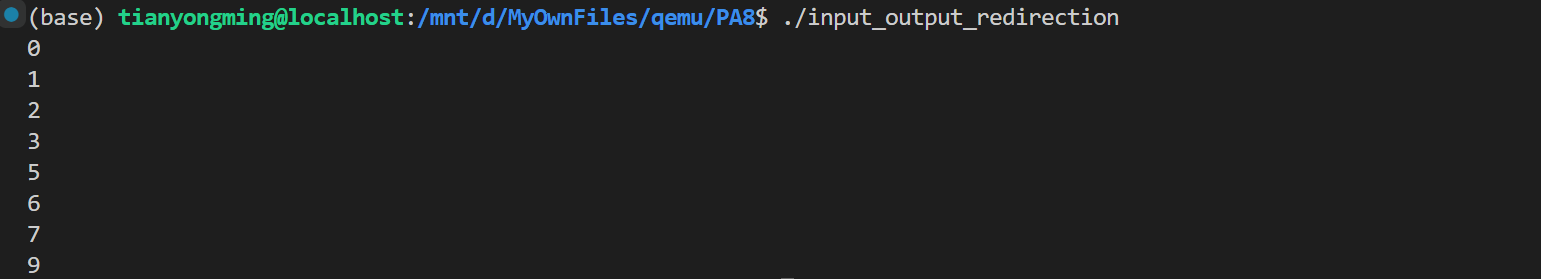
\includegraphics[width=\linewidth]{figures/my_output_true}
	\caption{}
	\label{fig:myoutputtrue}
\end{figure}

\begin{figure}[h!]
	\centering
	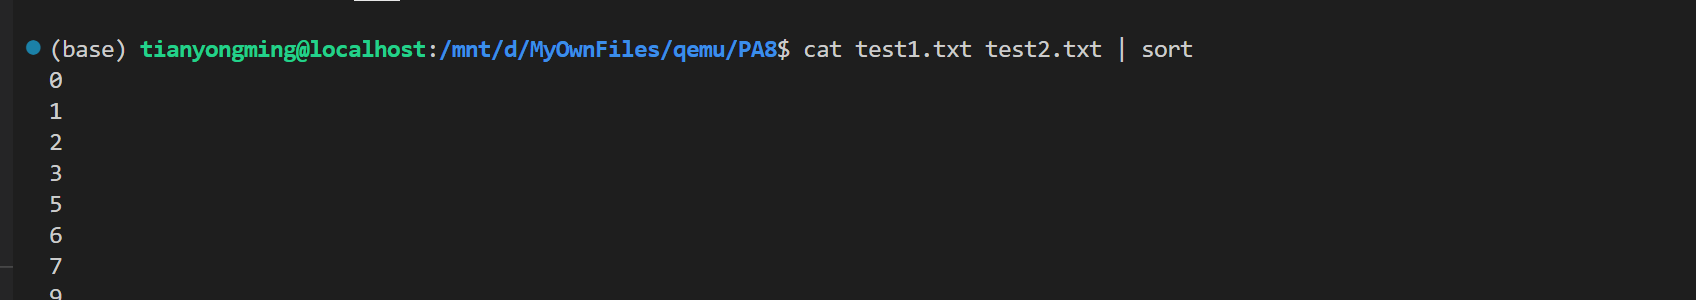
\includegraphics[width=\linewidth]{figures/standard_output}
	\caption{}
	\label{fig:standardoutput}
\end{figure}
	可以发现,结果是一致的,即正确的。
	
	\subsection{测试创建的匿名管道文件的容量限制的结果}
	测试结果如下:
	
\begin{figure}[h!]
	\centering
	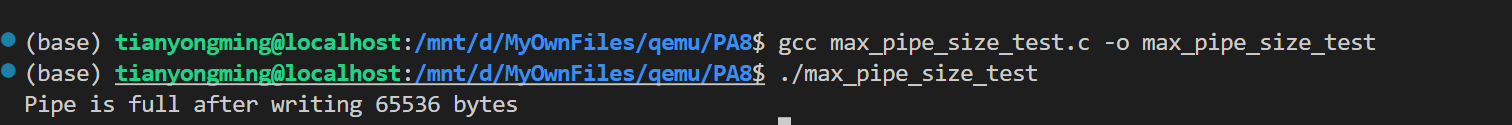
\includegraphics[width=1\linewidth]{figures/max_pipe_size}
	\caption{}
	\label{fig:maxpipesize}
\end{figure}

	由此可知,其最大容量为65536字节。也就是说,管道文件是由大小限制的,使用不当会出错。
	
	\section{总结与反思}
	\begin{itemize}
		\item 这次的实验,经过老师课上的讲解和伪代码的呈现,相对比较容易实现。实验中我只出现过一个问题,就是cat链接产生了错误输出,输出如下:
		
\begin{figure}[h!]
	\centering
	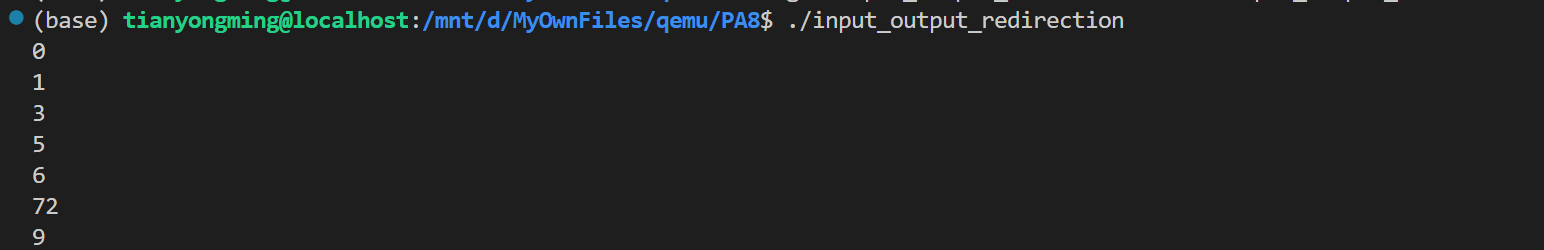
\includegraphics[width=1\linewidth]{figures/my_output_false}
	\caption{}
	\label{fig:myoutputfalse}
\end{figure}
�		这是由于我的test1.txt最后没有打换行,导致拼接的时候把7和test2.txt的2拼接成了一个数字。发现后,我增加了换行,解决了问题。
		\item 经过和老师讨论,我在这次实验基础上了解了管道同步机制,测试了匿名管道文件的最大容量,使得我对管道的理解更进一步。
		\item 老师课上并没有写关闭管道的不用的一端,但事实上这个操作是必要的,因为关闭管道不用的一端有助于防止意外的文件描述符泄漏。
	\end{itemize}

	\section{其它参考文献}
	除了正文给出的参考文献,我参考的文献还有:\par\hspace{0em}主要是徐锋老师的板书。
	
\end{document}
